\subsubsection{\stid{2.06} Exa-PAPI++}\label{subsubsect:exapapi}

\paragraph{Overview} 

%Understanding the performance characteristics of exascale applications is 
%necessary in order to identify and address the barriers to achieving performance 
%goals. This becomes more difficult as the architectures become more complex. 
%The Performance Application Programming Interface (PAPI) provides both library 
%and application developers with generic and portable access to low-level 
%performance counters found across the exascale machine, enabling users to see
%the relationships between software performance and hardware events. 
%These relationships provide a critical step toward improving performance.

The Exa-PAPI++ 
project is developing a new C++ Performance API (PAPI++) software package 
from the ground up that offers a standard interface and methodology for using
low-level performance counters in CPUs, GPUs, on/off-chip memory, interconnects, 
and the I/O system, including energy/power management. 
PAPI++ is building upon classic-PAPI functionality and strengthening its path to
exascale with a more efficient and flexible software design, one that takes 
advantage of C++'s object-oriented nature but preserves the low-overhead 
monitoring of performance counters and adds a vast testing suite.

In addition to providing hardware counter-based information, a standardizing layer 
for monitoring software-defined events (SDE) is being incorporated that exposes 
the internal behavior of runtime systems and libraries, such as communication and 
math libraries, to the applications. As a result, the notion of performance events is 
broadened from strictly hardware-related events to include software-based 
information. Enabling monitoring of both hardware and software events provides 
more flexibility to developers when capturing performance information.


\paragraph{Key Challenges}

Widely deployed and widely used, PAPI has established itself as fundamental
software infrastructure in every application domain where improving performance
can be mission critical. 
However, processor and system designs have been experiencing radical changes.
Systems now combine multi-core CPUs and accelerators, shared and
distributed memory, PCI-express and other interconnects, and
power efficiency is emerging as a primary design constraint.
These changes pose new challenges and bring new
opportunities to PAPI. At the same time, the ever-increasing importance of
communication and synchronization costs in parallel applications, as well as the
emergence of task-based programming paradigms, pose
challenges to the development of performance-critical applications and create a
need for standardizing performance events that originate from various ECP
software layers.


\paragraph{Solution Strategy}

The Exa-PAPI++ team is preparing PAPI support to stand up to 
the challenges posed by exascale systems by 
\begin{enumerate}
\item widening its applicability and providing robust support for exascale 
hardware resources;
\item supporting finer-grain measurement and control of power, thus offering 
software developers a basic building block for dynamic application optimization 
under power constraints; 
\item extending PAPI to support software-defined events; and 
\item applying semantic analysis to hardware counters so that the application 
developer can better make sense of the ever-growing list of raw hardware 
performance events that can be measured during execution. 
\end{enumerate}

%The Exa-PAPI effort delivers new PAPI components to handle the wide range of
%new hardware and software events for the extreme scale platforms that will form
%the basis of exascale computing. To achieve this, Exa-PAPI implements a variety
%of monitoring and sampling capabilities for the different technologies, which
%are exported to the ECP application community. 
%%
%Exa-PAPI also provides finer-grain measurement and control of power, thus
%offering software developers a basic building block for dynamic application
%optimization under power constraint. Other hardware efforts in Exa-PAPI are the
%development of components for monitoring network interconnect events, as well as
%components targeted at the deep and heterogeneous memory hierarchies that we
%are already seeing in new architectures.

In summary, the team will be channeling the monitoring capabilities of hardware 
counters, power usage, software-defined events into a robust PAPI++ software 
package. PAPI++ is meant to be PAPI's replacement---with a more flexible and 
sustainable software design.


\paragraph{Recent Progress}

On the \textbf{software event} front, the PAPI team has designed and implemented 
a new API to expose any kind of software-defined events. Since September 2019,
the SDE functionality is publicly available through the main repository of PAPI. 
As a result, software packages that reside in any layer of the software stack can now 
export information to the outside world in a uniform, well supported, and 
standardized way. 
 %
Since the concept of software-defined events is still new to PAPI, the team has worked
closely with developers of different ECP libraries and runtimes that serve as natural targets
for the adoption of the new SDE API.
As of today, we have integrated SDEs into the sparse linear algebra library MAGMA-Sparse 
(2.3.3.13 CLOVER), the tensor algebra library TAMM (2.2.1.02 NWChemEx), 
the task-scheduling runtime PaRSEC (2.3.1.09 PaRSEC), and the compiler-based 
performance analysis tool BYFL (2.4.2 HE). 

%\vspace{-4pt}
\begin{figure}[!h]
\begin{center}
  \subfloat[ ]{\label{fig:sde_magma}
  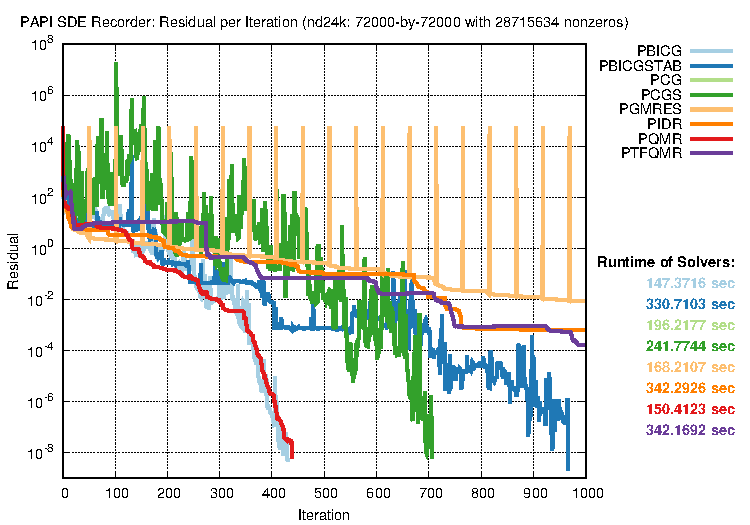
\includegraphics[width=0.49\linewidth]{projects/2.3.2-Tools/2.3.2.06-EXA-PAPI/Exa-PAPI_sde_magma.pdf}}
  \subfloat[ ]{\label{fig:sde_parsec}
  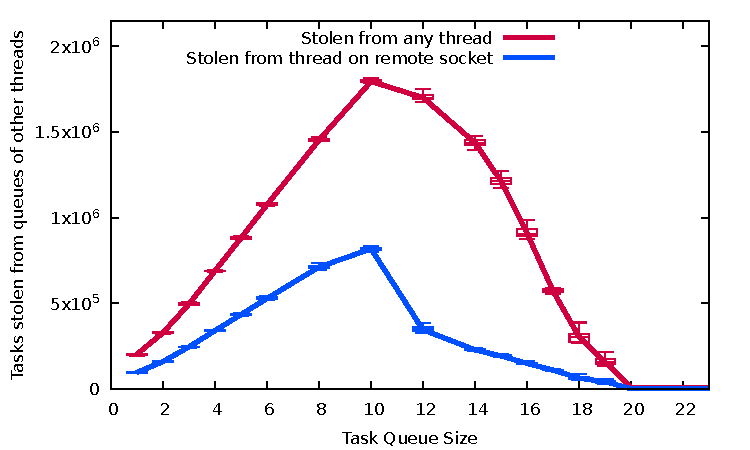
\includegraphics[width=0.49\linewidth]{projects/2.3.2-Tools/2.3.2.06-EXA-PAPI/Exa-PAPI_sde_parsec.pdf}}
%\vspace{-8pt}
\end{center}
\vspace{-9pt}
\caption{(a) PAPI SDE-Recorders log convergence of different ILU-preconditioned MAGMA-sparse Krylov solvers for a 2D/3D Problem; (b) PAPI SDEs count number of times the scheduler stole tasks from the task queue of another thread in PaRSEC.}
\end{figure}
%\vspace{-8pt}
%
%
The examples in Figure~\ref{fig:sde_magma} illustrate how the convergence of Krylov solvers can be
visualized with the help of PAPI SDEs. Each of these solvers behave very differently 
for different problems and matrices, which, once more, stresses the importance of 
\emph{exposing these details in a standardized way}. This allows the domain
scientist to quickly identify the fastest and most robust method of choice for 
their very unique problems. Most importantly, this information can now be obtained without 
expert knowledge about algorithm-specific characteristics,
and without having to instrument MAGMA library code, but simply by calling \verb+PAPI_read()+
in the top-level application.

Figure~\ref{fig:sde_parsec} serves as a second showcase, illustrating the evolution of 
task stealing during the execution of a PaRSEC application that is based on 
fork-join parallelism with 20 tasks generated at each fork.
With SDEs in PARSEC, a user can get a view of what is happening inside the runtime
by simply calling \verb+PAPI_start()+ and \verb+PAPI_stop()+ in their application, without the need to
instrument the PaRSEC runtime code. 


\vspace{10pt}
On the \textbf{hardware counter} front, we have developed support for the latest 
features on NVIDIA Volta GPUs (V100) as featured on the Summit and Sierra systems.
Specifically, PAPI users can now monitor both GPU hardware events and the NVLINK performance. 
Additionally, we developed PAPI capabilities for monitoring power consumption, fan speed, 
temperature, and power capping support for the V100 GPUs. 
The latest version of PAPI (5.7.0, released April 2019) has fully integrated support for the 
NVIDIA GPU counters and power management.
Similar efforts are currently in progress enabling users to monitor performance counters 
as well as power consumption on the AMD Vega GPUs.


\paragraph{Next Steps}

Our next efforts will focus on:
\begin{enumerate}
\item \textbf{Formulation of requirements for new PAPI C++ API:} 
		Create and circulate a survey to the ECP teams to assess their needs for hardware 
		and software performance counter functionality. Based on the survey results, 
		we will determine what features are needed for the new PAPI C++ interface. 
		Furthermore, perform a software requirement analysis, and explore novel concepts 
		for expressing software event and hardware counter 
		monitoring through the same PAPI C++ interface.
%
\item \textbf{Decompose PAPI's SDE functionality as standalone library}: 
		The SDE functionality will be decomposed from the PAPI package and made 
		available as a separate library. The production-ready version of the PAPI SDE 
		library will have fully integrated support for enabling SDEs in ECP software
		layers, as well as monitoring these new events through the PAPI interfaces.
%
\item \textbf{Formulation of a roadmap for refactoring traditional PAPI to PAPI++ software package}:
		Start the PAPI++ design process 
		for a modular framework that includes a new C++ API in addition to the traditional C 
		and Fortran APIs to preserve backward-compatibility. This effort involves a managed 
		transition away from our legacy PAPI software while continuing to add support for new 
		ECP hardware (released during FY20-21) until the official release of PAPI++.
\end{enumerate}
